\section{The Generic Architecture of Dresden OCL2 for Eclipse}
\label{sec:foundation}
	\note{try to be in-line with the terminology used in the abstract}

	\note{First motivate variation, adapt section heading accordingly}
	\note{explain required variability, feature model approach, resulting from
	related work on OCL applications, differentiate	 that vp1 and vp2 may vary
	independently in some cases, not in others..}
	\note{explain theory of ocl metalevel relativity  :) }
	\note{introduce variation points using Fig.2}
	
	
	\note{Fig 1. add headings to subfigures: a) Variation points in OCL Application	b) Applciation of OCL in UML modeling c) Application of OCL in Ecore
	metamodeling } 
	\note{Fig 1. can/should we change order to b), c) , a)? } 
	
	\begin{figure}[tb]
			\centering
				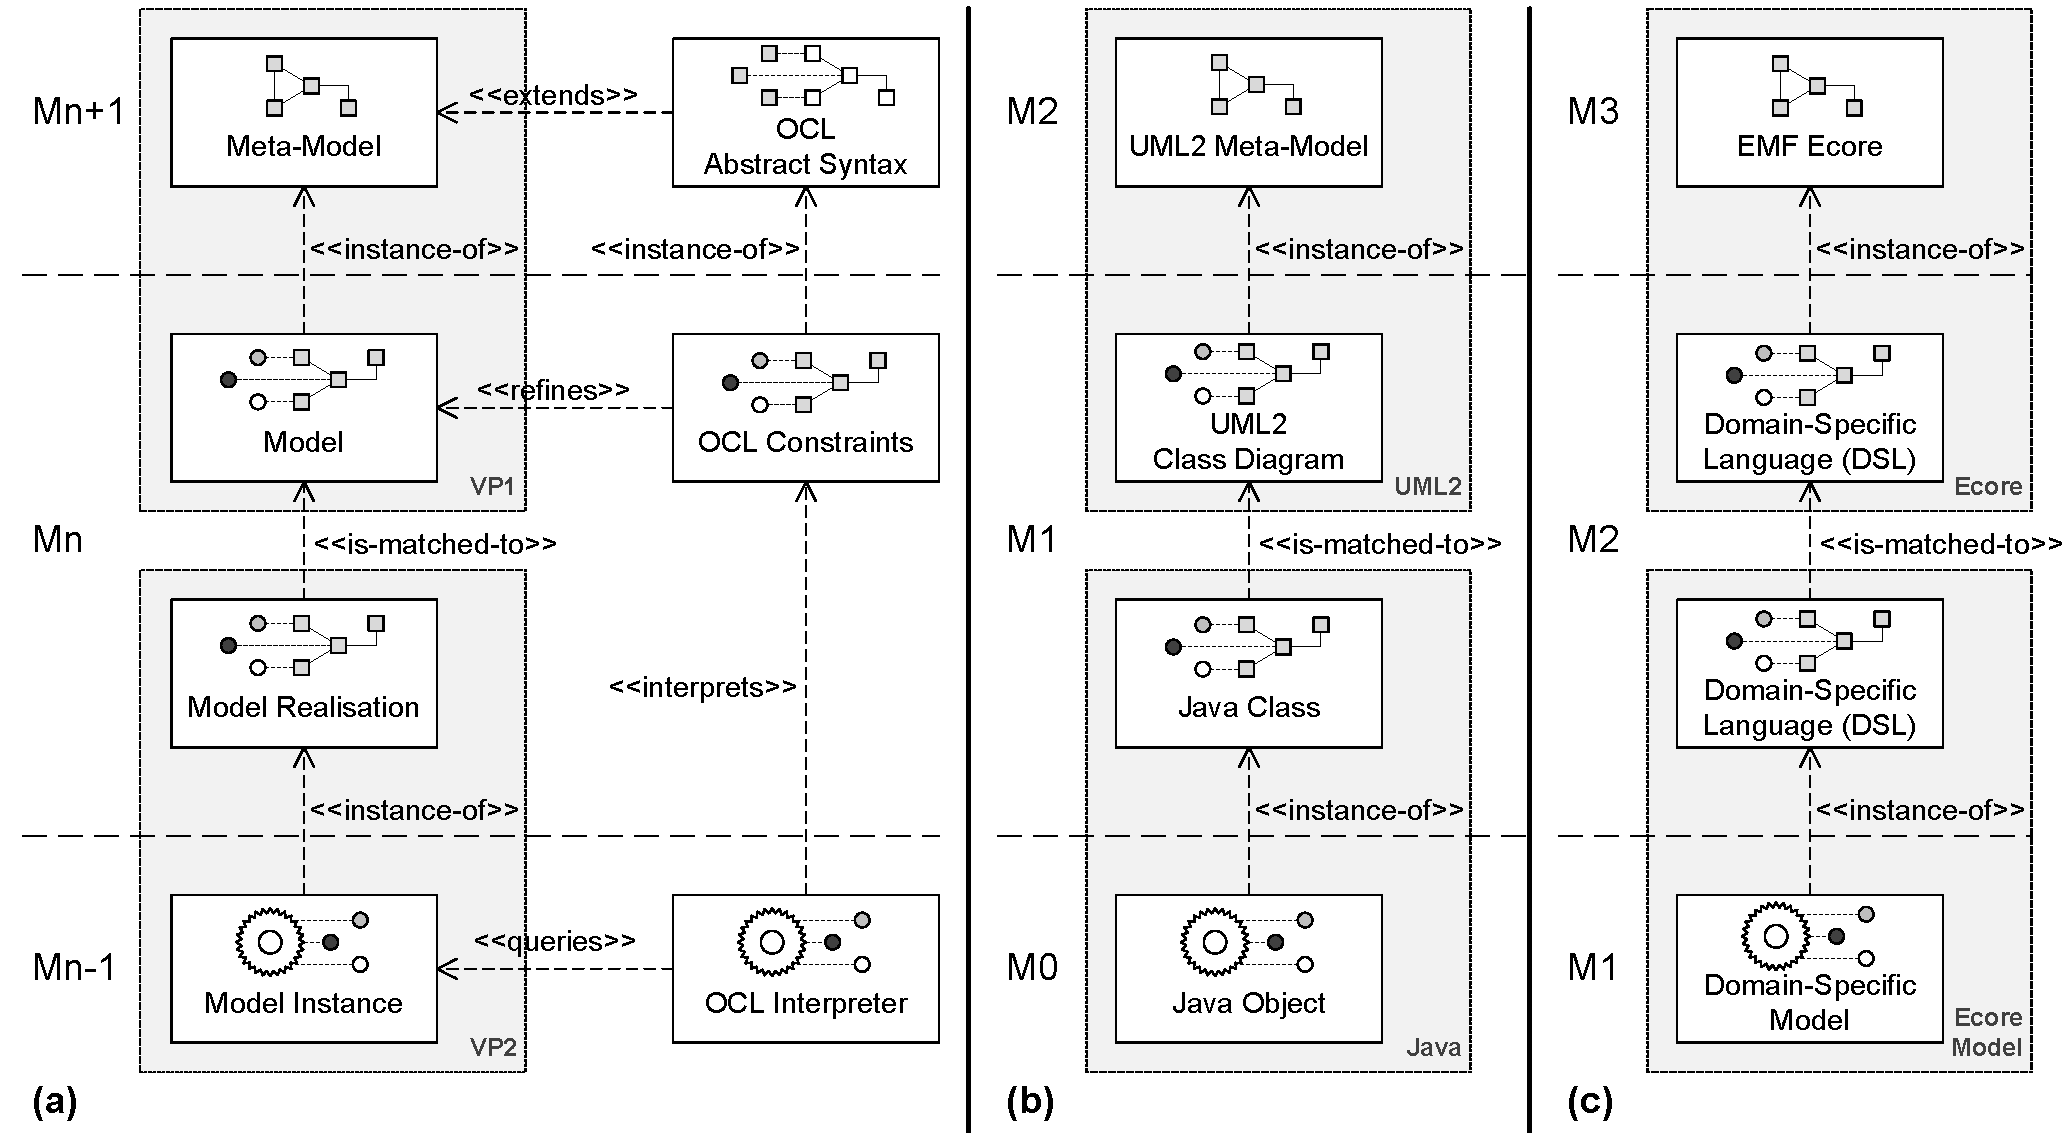
\includegraphics[width=1.00\textwidth]{figures/genericlayers.pdf}
			\caption{Variation Points in OCL Parsing and Interpretation}
			\label{fig:genericlayers}
		\end{figure}

\note{Michael: still too much caption text; in (b), is the UML2 meta-model
really MOF?, I thought MOF is on M3} The \textit{Generic Three Layer Meta data Architecture}. (a): Each OCL constraint requires a meta-model defining a model on which OCL constraints are specified. The 
			constraints are evaluated on a model instance that instantiates the constrained model. 
			The generic architecture can be parametrized at two different variation points. Different
			models and their meta-models can be bound to VP1, different model instances can be bound
			to VP2.	(b): UML-Example for layers M2, M1 and M0. VP1 is bound to the UML meta-model (MOF), 
			VP2 is bound to Java. (c): EMF-Example for layers M3, M2 and M1. VP1 is bound to EMF Ecore,
			VP2 is bound to Ecore-based models.

	To differentiate between meta-models, models and runtime objects, the OMG introduced 
	the \textit{MOF Four Layer Metadata Architecture}, that locates the meta-model, 
	model, and the model's instances at the layers \textit{M2}, \textit{M1} and \textit{M0}. 
	\note{Is that important to understand the paper?; Michael: agreed, just refer to it, but leave explaination}{Each language at layer
	\textit{Mn} is described in terms of a language resided at layer \textit{Mn-1}. Meta-meta-models 
	that are located at the layer \textit{M3} 
	can describe themselves reflexively.}
	
	Fig.~\ref{fig:genericlayers} depicts the \textit{Generic Three Layer
	Meta-Data Architecture} aligning OCL constraints with the MOF layers.
	\remove{As all
	models can be located in this layer architecture, OCL can be located there as
	well.} OCL constraints are a model and can be described using their abstract
	syntax, i.e., the OCL meta-model. They are evaluated for runtime objects at the 
	model instance layer. 
	%\remove{Thus, three layers must be known by the OCL tool
	%to define and evaluate the constraints. This notion leads to the 
	%Generic Three Layer Meta-Data Architecture demuthRGWS09} that 
	%allows to define an OCL tool independently of specific layers. As can be seen
	%in Figure \ref{fig:genericlayers} the OCL model (all constraints) enriches
	%another model.} 
	In order to \change{navigate through the  model or to call
	operations on}{define constraints on models OCL needs to navigate on} model
	elements. To bind OCL constraints on the navigation structure in
	the model they are defined on, the abstract syntax of OCL
	\note{this is true for UML, but sounds quite technical}{extends} the model's
	meta-model.
	%OCL can be used to define well-formedness rules, i.e., constraints on meta-models (M2) that are evaluated at the model level (M1), or business rules, i.e., constraints defined on models (M1) that are evaluated for runtime objects at the model instance layer (M0).
	
	\note{we need to incorporate the motivation for implementation language
	variation here. Reviewers need to understand the problem to understand our
	solution.}


	\note{This section does not clarify the contribution of THIS paper. We should
	sell the instance adaptation as a improvement of previous DresdenOCL versions

		\begin{itemize}
		  \item motivation: different model implementations are useful
		  \item context: identify variation points in fig 1, modeling langauge,
		  implementation language
		  \item problem: neither dresdenOCL nor others are able to cope with differnt
		  model implementations
		  \item solution: we suggest additional adaptation interface
		  \item feasibility: we contribute implementation of adaptation approach in
		  Dresden OCL
		\end{itemize}
	
	}

	{The architecture of Dresden OCL2 for Eclipse was developed in respect to the 
	generic three layer meta-data architecture. In order to reuse the developed 
	OCL tools, DresdenOCL does not directly accesses models or model instance objects. 
	Instead, these are hidden behind a common set of interfaces that delegate to 
	their adaptee. The adaption of models and model instance objects is presented 
	in the following.}
